\begin{song}{title=\predtitle \centering Nic není tak horký \\\large Bratři Ebenové \vspace*{-0.5cm}}  %% sem se napíše jméno songu a autor
\vspace*{.5cm}

\moveright -.5cm \vbox{
\begin{centerjustified}
\velky

\begin{varwidth}[t]{0.5\textwidth}\setlength{\parindent}{\pindent}  %Varianta č. 2 --> Dva sloupce

\sloka
^{Emi}Znáš to, ^{Emi6/H \z}jak~to~chodí,

^{Emi Emi6/H Emi7/A}pokaždé~se~neurodí.

^{Emi}Znáš to, ^{Emi6/H \z}jak~to chodí.

\writechord{Emi Emi6/H Emi7/A}

^{Emi}Znáš to, ^{Emi6/H \z}jak~to~bývá,

^{Emi Emi6/H Emi7/A \z}rána~jsou~nelichotivá.

^{Emi}Znáš to, ^{Emi6/H \z}jak~to bývá.

\writechord{Emi Emi6/H Emi7/A Cmaj7}


\sloka
Jenomže ^{G}nic není tak horký, jak se ^{C \z}upeče.

A ^{G \z}každá kalná voda jednou ^{C \z}odteče.

A ^{Emi \z}každý chladný ^{Hmi \z}vítr jednou ^{Ami \z}dofičí.

A každá ^{D9 \z}mánička jde někdy k ^{D7 \z}holiči.

I ^{G \z}oceán má někde svoje ^{Cmaj7 \z}okraje.

A i ^{G \z}nejdelší deska jednou ^{Cmaj7 \z}dohraje.

I ^{Emi \z}dálný východ ^{Hmi \z}není zas tak ^{Ami \z}daleký.

A jenom ^{D9 \z}láska ta vytrvá ^{\z G\,}navěky.

\writechord{C Emi A}

\end{varwidth}\mezisloupci\begin{varwidth}[t]{0.6\textwidth}\setlength{\parindent}{\pindent}

\sloka
Znáš to, to se stává,

když se příběh zadrhává.

Znáš to, to se stává,

pryč jsou všechna slova.

Čas je dávno vygumoval,

pryč jsou všechna slova.


\sloka
Jenomže každý velký požár jednou dohoří.

A každá zeď se jednoho dne rozboří.

A každý metál jednou spadne ze hrudi.

A každý prudič jednoho dne doprudí.

A každý bohém jednou skončí v papučích.

A každý blb se někdy něco naučí.

A každý muslim jednou dojde do Mekky.

A jenom láska ta vytrvá.


\sloka
A bohatí nebudou vždycky bohatí.

A každé platidlo po čase doplatí.

A každé zboží jednou skončí na pultu.

A každý docent najde svoji fakultu.

A i moře se jednoho dne umoří.

Až srovnají se propasti i pohoří.

A přikryje nás prach tak jako Aztéky.

A jenom láska ta vytrvá navěky.

\mezera

\centering
\includefret{Emi}
\includefret{Emi6-H}
\includefret{Emi7-A}

\includefret{Dsus2}
\includefret{D7}
\includefret{Cmaj7}

\end{varwidth}
\end{centerjustified}
}

\centering
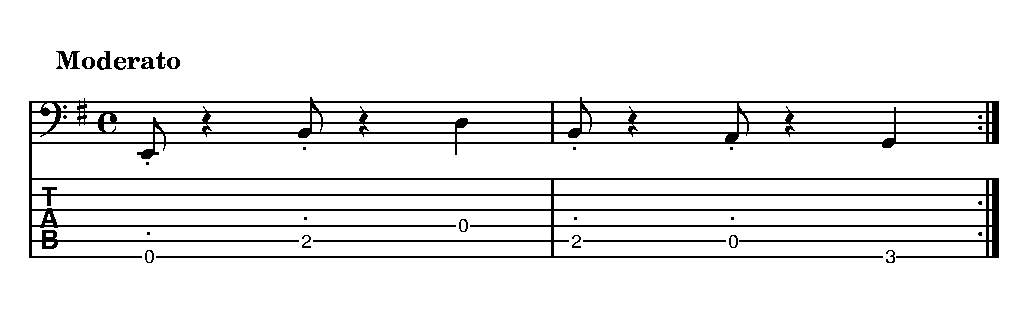
\includegraphics[scale=\defaulttabscale]{../taby/nicnenitakhorky.pdf}

\setcounter{Slokočet}{0}
\end{song}
    
